\documentclass{article}

% various packages and settings {{{

% math packages
\usepackage{amsmath, amsfonts, mathtools}

% other important packages (should stay on top)
\usepackage{graphics, multicol, xcolor}

% change to German
\usepackage[german]{babel}

% utf8 characters
\usepackage[utf8]{inputenc}

% font
\usepackage[scaled]{helvet}
\renewcommand{\familydefault}{\sfdefault}
\usepackage[]{fontspec}

% set title spacing
% titlesec above hyperref, else conflict
\usepackage{titlesec}
\titlespacing\section{0pt}{12pt}{0pt}
\titlespacing\subsection{0pt}{12pt}{0pt}
\titlespacing\subsubsection{0pt}{12pt}{0pt}

% links
\usepackage{hyperref}
\hypersetup{
    colorlinks,
    citecolor=black,
    filecolor=black,
    linkcolor=black,
    urlcolor=black
}

% fontsize
\usepackage[12pt]{extsizes}

% no paragraph indents
\setlength{\parindent}{0pt}

% better hyphenation
\usepackage[final]{microtype}
\usepackage{csquotes}

% import line spacing
\usepackage{setspace}

% page format
\usepackage{geometry}
\geometry{
    a4paper,
    left=25mm,
    right=25mm,
    top=15mm,
    bottom=25mm
}

% colorful boxes
\usepackage{mdframed}

\setcounter{secnumdepth}{0} % no section numbering
% }}}

% custom commands {{{
\usepackage{environ}

% define custom formula environment
\NewEnviron{formulas}{
    \vspace{-2.5em}
    \Large
    \begin{align*}
        \BODY
    \end{align*}
    \normalsize
}

% same formula env, but with red border
\NewEnviron{Formulas}{
    \begin{mdframed}[linecolor=red]
        \vspace{-2.5em}
        \Large
        \begin{align*}
            \BODY
        \end{align*}
        \normalsize
    \end{mdframed}
}

% normal-sized text inside the formulas
\newcommand{\normaltext}[1]{
    \normalsize\text{#1}\Large
}

% }}}

% figures
\usepackage{float}
\usepackage{caption}
\captionsetup{labelformat=empty}

% scaling
\usepackage{adjustbox}

% tikz
\usepackage{tikz}
\usepackage{tkz-euclide}
\usetikzlibrary{arrows.meta}

\begin{document}

\addtocounter{page}{-3}
\setstretch{1.5}

\title{Mathematik 12/13 Niedersachsen}
\date{\today}
\author{}
\maketitle

\thispagestyle{empty}

\clearpage

\pagestyle{empty}

\tableofcontents

\clearpage

\pagestyle{plain}

% ------------ Vektoren, Geraden, Ebenen, Abstände im Raum ------------ %
\section{Vektoren}

Ein Vektor beschreibt eine Verscheibung mit Richtung im Raum.
Ein Vektor kann von jedem Ort im Raum ausgehen und kann dann einen Start- und Endpunkt haben.
Jeder Punkt im Raum lässt sich mit einem Vektor vom Ursprung $O$ zu den
Koordinaten des Punktes beschreiben.

\begin{equation*}
    \vec{v} = \begin{bmatrix}
        5 \\
        3 \\
        7
    \end{bmatrix}
    \qquad A (1, 2, 2) \; B (4, 3, 1) \rightarrow \vec{AB} = \begin{bmatrix}
        3 \\
        1 \\
        -1
    \end{bmatrix}
    \qquad P (1, 3, 2) \rightarrow \vec{OP} = \begin{bmatrix}
        1 \\
        3 \\
        2
    \end{bmatrix}
\end{equation*}

\subsection{Rechnen mit Vektoren}

\subsubsection{Addition und Subtraktion}

Bei beim Rechnen mit Vektoren werden die Komponenten des einen Vektors
mit den Komponenten des anderen Vektors addiert bzw. subtrahiert.
Multiplikation ist dabei auf verschiedene Arten (später erklärt) möglich.
Division ist nicht möglich.

\begin{equation*}
    \begin{bmatrix}
        3 \\
        1 \\
        -2
    \end{bmatrix}
    +
    \begin{bmatrix}
        2 \\
        3 \\
        1
    \end{bmatrix}
    =
    \begin{bmatrix}
        5 \\
        4 \\
        -1
    \end{bmatrix}
    \qquad
    \begin{bmatrix}
        3 \\
        1 \\
        -2
    \end{bmatrix}
    -
    \begin{bmatrix}
        2 \\
        3 \\
        1
    \end{bmatrix}
    =
    \begin{bmatrix}
        1 \\
        -2 \\
        -3
    \end{bmatrix}
\end{equation*}

\subsubsection{Länge eines Vektor}

Die Länge eines Vektors ergibt sich aus dem Satz des Pythagoras.
Betragsstriche um einen Vektor bedeuten, dass dessen Länge gemeint ist.

\begin{equation*}
    \vec{AB} = \begin{bmatrix}
        3 \\
        1 \\
        -1
    \end{bmatrix}
    \qquad | \vec{AB} | = \sqrt{3^2 + 1^2 + (-1)^2} = \sqrt{11}
\end{equation*}

\subsubsection{Gegenvektor}

Der Gegenvektor ist die Umkehrung eines Vektors.

\begin{equation*}
    \vec{v} =
    \begin{bmatrix}
        3 \\
        -1 \\
        2
    \end{bmatrix}
    \qquad \vec{v} \cdot -1 = \vec{g} =
    \begin{bmatrix}
        -3 \\
        1 \\
        -2
    \end{bmatrix}
\end{equation*}

\subsubsection{Vektoren mit Vorfaktor}

Hat ein Vektor einen Vorfaktor (Skalar), so ist jede Komponente
des Vektors mit diesem zu multiplizieren.

\begin{equation*}
    2 \cdot
    \begin{bmatrix}
        3 \\
        -1 \\
        2
    \end{bmatrix}
    =
    \begin{bmatrix}
        6 \\
        -2 \\
        4
    \end{bmatrix}
\end{equation*}

\subsection{Kollineare Vektoren}

Vektoren sind kollinear, wenn sich der eine Vektor aus der Multiplikation
des anderen Vektors mit einem Skalar ergibt.
Sind zwei Vektoren kollinear, so bedeutet dies, dass beide die gleiche
Richtung beschreiben.

\begin{equation*}
    \vec{a} =
    \begin{bmatrix}
        4 \\
        6 \\
        2
    \end{bmatrix}
    \qquad
    \vec{b} =
    \begin{bmatrix}
        2 \\
        3 \\
        1
    \end{bmatrix}
    \qquad
    \vec{a} =
    2 \cdot \vec{b} =
    2 \cdot
    \begin{bmatrix}
        2 \\
        3 \\
        1
    \end{bmatrix}
    =
    \begin{bmatrix}
        4 \\
        6 \\
        2
    \end{bmatrix}
\end{equation*}

\subsection{Abstand von Punkten}

Um die Distanz zwischen zwei Punkten bzw. den Endpunkten von 2 vom gleichen Ort
ausgehenden Vektoren zu berechnen, muss nur die Länge des Differenzvektors berechnet
werden. Die Länge von $\vec{d}$ ist somit der Abstand zwischen
$\vec{v_1}$ und $\vec{v_2}$.
Eine Formel lässt sich somit von der Längenformel eines Vektors ableiten.

\begin{equation*}
    \vec{v_1} =
    \begin{bmatrix}
        4 \\
        6 \\
        2
    \end{bmatrix}
    \quad
    \vec{v_2} =
    \begin{bmatrix}
        1 \\
        2 \\
        0
    \end{bmatrix}
    \quad
    \vec{d} =
    \begin{bmatrix}
        3 \\
        4 \\
        2
    \end{bmatrix}
    \quad
    \begin{aligned}
        | \vec{d} | & = \sqrt{(x_1 - x_2)^2 + (y_1 - y_2)^2 + (z_1 - z_2)^2} \\
        | \vec{d} | & = \sqrt{(4 - 1)^2 + (6 - 2)^2 + (2 - 0)^2}
    \end{aligned}
\end{equation*}

\subsection{Mittelpunkt einer Strecke}

\subsection{Skalarprodukt}

Das Skalarprodukt ist die Summe der Produkte der einzelnen Vektorelemente.
Das Ergebnis ist eine relle Zahl.

\begin{equation*}
    \begin{bmatrix}
        3 \\
        1 \\
        -1
    \end{bmatrix} \cdot
    \begin{bmatrix}
        2 \\
        0 \\
        -1
    \end{bmatrix} = 3 \cdot 2 + 1 \cdot 0 + -1 \cdot -1 = 7
\end{equation*}

\subsubsection{Winkel beim Skalarprodukt}

Für den Winkel zwischen 2 vom gleichen Punkt ausgehenden Vektoren gelten folgende Formeln
Ist das Skalarprodukt gleich 0, so sind die Vektoren orthogonal, ist dass Skalarprodukt
gleich des Produkts der Vektorlängen, so sind die Vektoren kollinear.

\begin{equation*}
    \cos (\alpha) = \frac{\vec{a} \cdot \vec{b}}{|\vec{a}| \cdot |\vec{b}|}
    \qquad \vec{a} \cdot \vec{b} = 0 \Rightarrow \alpha = 90°
    \qquad \vec{a} \cdot \vec{b} = |\vec{a}| \cdot |\vec{b}| \Rightarrow \alpha = 0°
\end{equation*}

\subsubsection{Skalarprodukt: Assoziativ, Kommutativ und Distributiv}

Beim Skalarprodukt gelten die Rechengesetze Assoziativgesetz, Kommutativgesetz und Distributivgesetz.

\begin{equation*}
    \vec{a} \cdot \vec{b} = \vec{b} \cdot \vec{a}
    \qquad (\vec{a} \cdot \vec{b}) \cdot \vec{c} = \vec{a} \cdot (\vec{b} \cdot \vec{c})
    \qquad (\vec{a} + \vec{b}) \cdot \vec{c}  = \vec{a} \cdot \vec{c} + \vec{b} \cdot \vec{c} 
\end{equation*}

\subsection{Kreuzprodukt}

Das Kreuzprodukt zweier Vektoren ergibt einen dritten Vektor der orthogonal
zu beiden anderen ist. Das Kreuzprodukt von Rot-Blau ist der Vektor Pink, orthogonal zur
Ebene von Rot-Blau.

\begin{equation*}
    \vec{a} \times \vec{b} =
    \begin{bmatrix}
        a_1 \\
        a_2 \\
        a_3
    \end{bmatrix} \times
    \begin{bmatrix}
        b_1 \\
        b_2 \\
        b_3
    \end{bmatrix} =
    \begin{bmatrix}
        a_2 b_3 - a_3 b_2 \\
        a_3 b_1 - a_1 b_3 \\
        a_1 b_2 - a_2 b_1
    \end{bmatrix}
    \qquad
    \begin{bmatrix}
        3 \\
        1 \\
        -1
    \end{bmatrix} \times
    \begin{bmatrix}
        2 \\
        0 \\
        -1
    \end{bmatrix} =
    \begin{bmatrix}
        1 \cdot (-1) - (-1) \cdot 0 \\
        (-1) \cdot 2 - 3 \cdot (-1) \\
        3 \cdot 0 - 1 \cdot 2
    \end{bmatrix} =
    \begin{bmatrix}
        -1 \\
        1 \\
        -2
    \end{bmatrix}
\end{equation*}

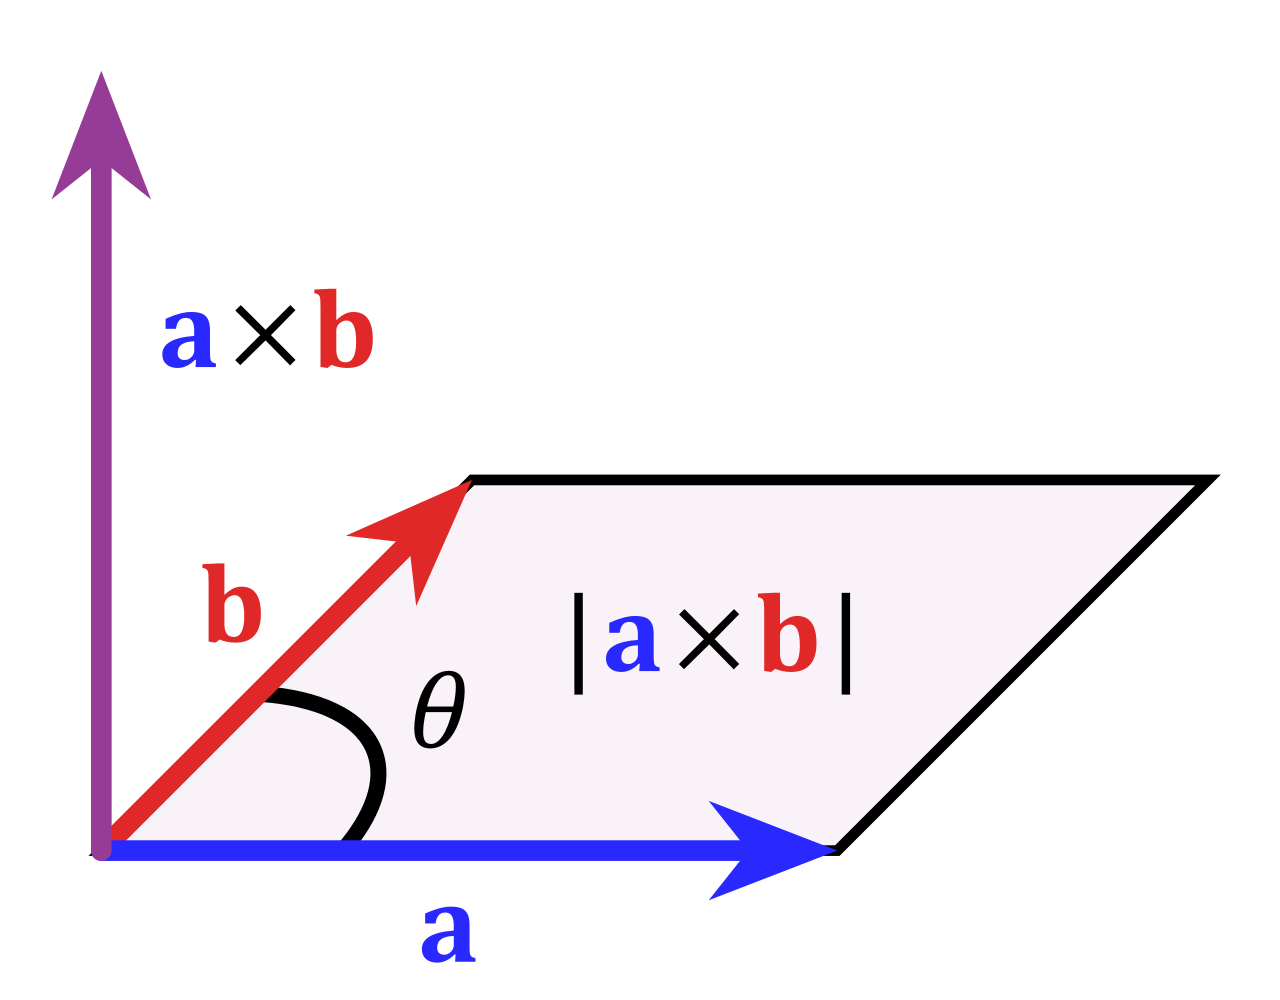
\includegraphics[width=0.4\textwidth]{images/cross-p.png}


\section{3D Koordinatensystem}

Die Darstellung eines 3D-Koordinatensystems in 2D (z. B. als Zeichnung auf Papier)
ist mit verschiedenen Abmessungen möglich. Außerdem ist es beim Punkte einzeichnen nötig,
strikt die Reihenfolge x, y, z einzuhalten.
Beim Ablesen von Punkten muss 1 Koordinate des Punktes bereits bekannt sein, da die Punkte
sonst mehrdeutig sind. Diese Angabe ist allerdings nicht immer explizit gegeben,
sondern ergibt sich meist aus dem Zusammenhang (z. B. von einer Aufgabe).

\begin{figure}[H]
    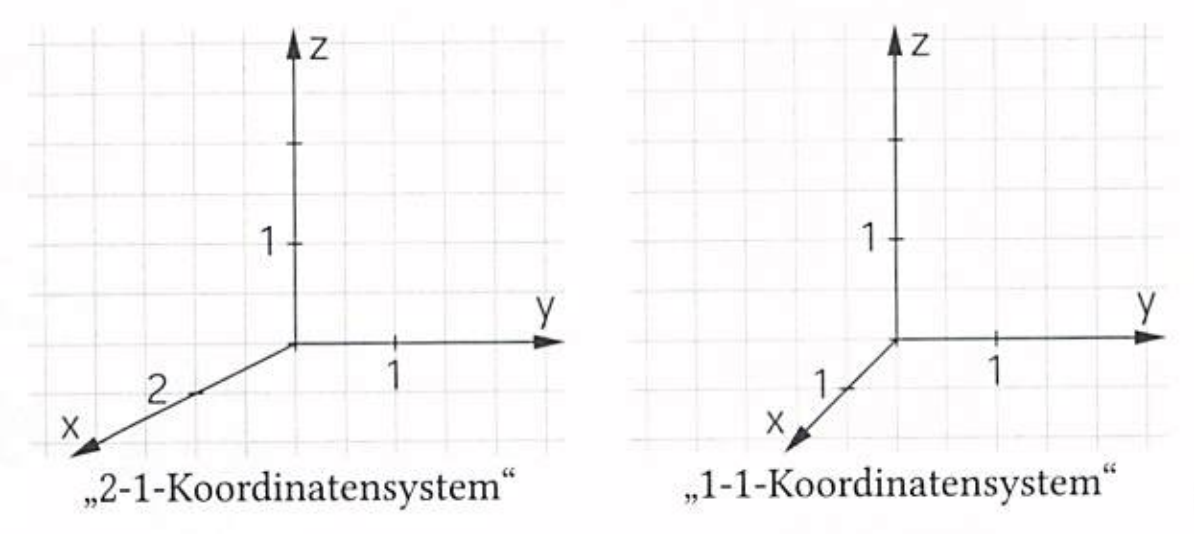
\includegraphics[width=0.8\textwidth]{images/3d-cord-systems.png}
    \caption{3D Koordinatensystem Arten}
\end{figure}

\begin{figure}[H]
    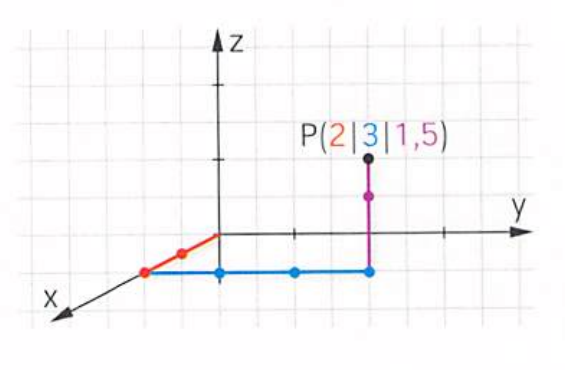
\includegraphics[width=0.6\textwidth]{images/3d-draw-point.png}
    \caption{Einzeichen von P(2 | 3 | 1,5)}
\end{figure}

\section{Geraden}
\subsection{Geradengleichung}

Eine Gerade im 3-dimensionalen Raum ist vergleichbar mit einer linearen Funktion im einem 2-dimensionalen
Koordinatensystem. Bei einer Gerade gibt es einen Startpunkt (vgl. y-Achsenabschnitt)
und eine Richtung (vgl. Steigung). Der Startpunkt wird Stützvektor genannt und beschreibt einen
Punkt im Raum. Die Richtung wird vom Richtungsvektor beschrieben. Da die Gerade im Raum
liegt, bestehen alle Koordinaten aus 3 Werten (also x, y, z).

\begin{equation*}
    g: \vec{x} = \vec{a} + r \cdot \vec{v}
    \qquad g: \vec{x} =
    \begin{bmatrix}
        2 \\
        1 \\
        3
    \end{bmatrix}
    +
    r \cdot
    \begin{bmatrix}
        1 \\
        1 \\
        2
    \end{bmatrix}
\end{equation*}

Eine Geradengleichung lässt sich aus 2 Punkten aufstellen. Einer der Punkte wird der
Stützvektor und der Richtungsvektor der Geraden ist der Differenzvektor der beiden Punkte.
Eine Gerade durch die Vektoren (Punkte) $\vec{c}$ und $\vec{d}$ wäre wie folgt.

\begin{equation*}
    \begin{aligned}
        \vec{a} & = \vec{c} \\
        \vec{v} & = \vec{c} - \vec{d}
    \end{aligned}
    \qquad g: \vec{x} = \vec{a} + r \cdot \vec{v}
\end{equation*}

Eine Gerade kann dabei durch Unendlich viele unterschiedliche Geradengleichungen
beschrieben werden, da jeder Punkt auf der Gerade als Stützvektor dienen kann
und da alle zum Richtungsvektor kollinearen Vektoren auch die gleiche Gerade
beschreiben.

\subsection{Spurpunkte auf Koordinatenebenen}

Eine Gerade kann 1, 2 oder 3 der Koordinatenebenen jeweils in einem Punkt schneiden.
Diese Punkte nennt man dann Spurpunkte. Ob eine Gerade eine bestimmte Koordinatenebene
schneidet lässt sich dadurch feststellen, dass für einen Wert $r$ die nicht zur Ebene
gehörende Koordinate gleich 0 ist. Eine Schnittpunkt einer Gerade in $P(10 | 0 | 10)$ würde
einen Spurpunkt auf der x-z Ebene bedeuten, da die y Koordinate gleich 0 ist.

\vspace*{0.2cm}

Für eine Gerade $g$ lässt sich z. B. der Spurpunkt der y-z Ebene bestimmten.
Die zu erfüllende Bedingung ist $x = 0$, die anderen Koordinaten sind egal.
Durch dass Komponentenweise gleichsetzen von Vektor und Geradengleichung lässt
sich, wenn es einen Spurpunkt gibt, der Wert von $r$ bestimmen, wenn dies der Fall ist.
Dazu muss die Gleichung der der auf 0 gesetzten Koordinate gelöst werden. 

\begin{equation*}
    g: \vec{x} =
    \begin{bmatrix}
        2 \\
        1 \\
        3
    \end{bmatrix}
    +
    r \cdot
    \begin{bmatrix}
        1 \\
        1 \\
        2
    \end{bmatrix}
    \qquad
    \begin{bmatrix}
        0 \\
        y \\
        z
    \end{bmatrix}
    =
    \begin{bmatrix}
        2 \\
        1 \\
        3
    \end{bmatrix}
    +
    r \cdot
    \begin{bmatrix}
        1 \\
        1 \\
        2
    \end{bmatrix}
    \qquad
    \begin{aligned}
        0 = 2 + r \cdot 1 \\
        \Rightarrow r = -2
    \end{aligned}
    \qquad
    \vec{s} =
    \begin{bmatrix}
        0 \\
        -1 \\
        -1
    \end{bmatrix}
\end{equation*}

\subsection{Lagebeziehungen von Geraden}
\subsubsection*{Geraden liegen parralel}

Die Geraden liegen parallel, wenn die Richtungsvektoren kollinear sind.

\subsubsection*{Geraden sind identisch}

Die Geraden sind identisch, wenn die Richtungsvektoren kollinear sind und
der Stützvektor der 1. Geraden auf der 2. Gerade liegt.
Dies lässt sich durch gleichsetzen von Stützvektor und Geradengleichung prüfen.

\subsubsection*{Geraden schneiden sich}

Die Geraden schneiden sich, wenn die Richtungsvektoren nicht kollinear sind
und für ein Wertepaar $r_1, r_2$ (Faktoren der Geradengleichungen) die Geradengleichungen
den gleichen Punkt beschreiben. Dies lässt sich durch gleichsetzen von 2 Geradengleichungen
überprüfen (Sind die Geraden identisch, so gibt es unendlich viele Wertepaare).
Daraus entsteht dann ein Gleichungssystem, was sich mit Hilfsmitteln (Taschenrechner)
oder von Hand lösen lässt.

\begin{align*}
    \vec{p} + r_1 \cdot \vec{u} = \vec{q} + r_2 \cdot \vec{v} \Rightarrow \\
    \\
    p_1 + r_1 \cdot u_1 = q_1 + r_2 \cdot v_1 \\
    p_2 + r_1 \cdot u_2 = q_2 + r_2 \cdot v_2 \\
    p_3 + r_1 \cdot u_3 = q_3 + r_2 \cdot v_3 \\
\end{align*}

\subsubsection*{Geraden liegen windschief}

Um zu überprüfen, ob die Geraden windschief liegen, muss versucht werden, ein Schnittpunkt
zu berechnen. Ergibt sich kein Schnittpunkt, so liegen die Geraden windschief.

\section{Ebenen}
\subsection{Ebenenformen}
\subsubsection{Parameterform}
\subsubsection{Normalenform}
\subsubsection{Koordinatenform}
\subsubsection{Umwandlung zwischen den Formen}
\subsection{Punktprobe für Ebenen}
\subsection{Lagebeziehung Gerade-Ebene}
\subsubsection{Schnittpunkt Gerade-Ebene}
\subsubsection{Gerade parallel zur Ebene}
\subsubsection{Gerade liegt in der Ebene}
\subsection{Lagebeziehung Ebene-Ebene}
\subsubsection{Schnittgerade}
\subsubsection{Ebenen liegen parralel}
\subsubsection{Ebenen liegen ineinander}
\subsection{Winkel zwischen Geraden und Ebenen}
\subsubsection{Winkel Gerade-Gerade}
\subsubsection{Winkel Gerade-Ebene}
\subsubsection{Winkel Ebene-Ebene}

\subsection{Abstände im Raum}
\subsubsection{Abstand Punkt-Gerade (Analysis)}
\subsubsection{Abstand Punkt-Gerade (Skalarprodukt)}
\subsubsection{Abstand Punkt-Ebene}
\subsubsection{Abstand windschiefer Geraden}
\subsubsection{Abstände bei parallelen Geraden und Ebenen}

\clearpage

\section{Spiegelungen}

\subsection{2D Spiegelungen}

Achsenspiegelung und Punktspiegelung im 2-dimensionalen Raum.

\begin{figure}[H]
    \adjustbox{scale=0.8}{
    \begin{tikzpicture}
        % system
        \tkzInit[xmin=-4,xmax=4,ymin=-4,ymax=4]
        \tkzGrid
        \draw [thick,->] (-4.5, 0) -- (4.5, 0);
        \draw [thick,->] (0, -4.5) -- (0, 4.5);
        \node at (4.5, -0.5) {x};
        \node at (-0.5, 4.5) {y};
        % vectors, points
        \draw[red, arrows = {-Stealth}] (0, 2) -- (2.9, 2);
        \draw[red, arrows = {-Stealth}] (0, 2) -- (-2.9, 2);
        \draw[blue] (0, -4) -- (0, 4);
        \draw [color=blue, fill=green] (3, 2) circle (0.05);
        \draw [color=blue, fill=green] (-3, 2) circle (0.05);
    \end{tikzpicture}
    }
    \adjustbox{scale=0.8}{
    \begin{tikzpicture}
        % system
        \tkzInit[xmin=-4,xmax=4,ymin=-4,ymax=4]
        \tkzGrid
        \draw [thick,->] (-4.5, 0) -- (4.5, 0);
        \draw [thick,->] (0, -4.5) -- (0, 4.5);
        \node at (4.5, -0.5) {x};
        \node at (-0.5, 4.5) {y};
        % vectors, points
        \draw[red, arrows = {-Stealth}] (0, 0) -- (2.9, 2);
        \draw[red, arrows = {-Stealth}] (0, 0) -- (-2.9, -2);
        \draw [color=blue, fill=green] (3, 2) circle (0.05);
        \draw [color=blue, fill=green] (-3, -2) circle (0.05);
        \draw [color=blue, fill=blue] (0, 0) circle (0.1);
    \end{tikzpicture}
    }
\end{figure}

\subsection{3D Spiegelungen}

Punktspiegelung, Ebenenspiegelung und Achsenspiegelung im 3-dimensionalen Raum.

\begin{figure}[H]
    \centering
    \setkeys{Gin}{width=0.3\linewidth}
    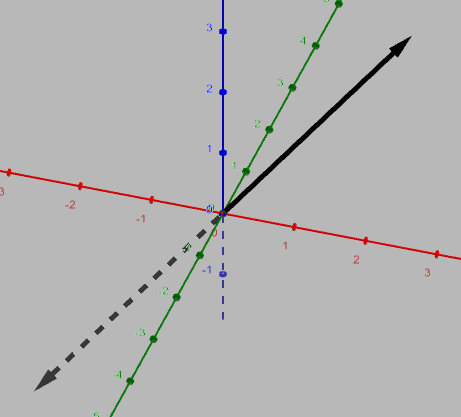
\includegraphics[width=0.3\textwidth]{images/3d-point-reflection.png} \,
    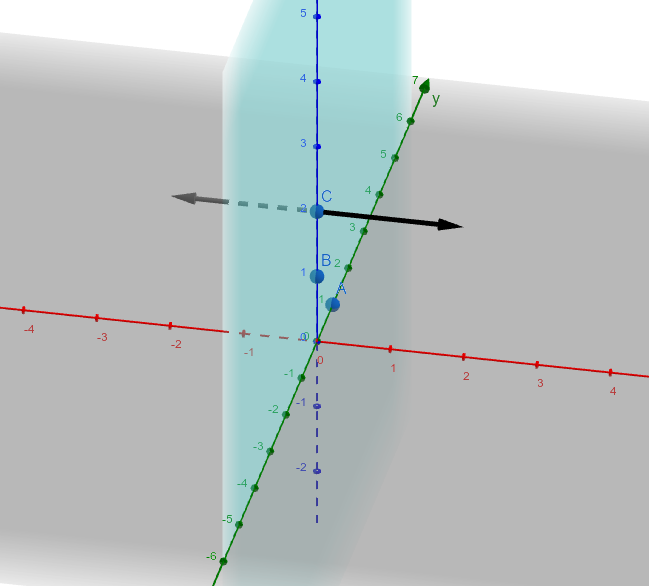
\includegraphics[width=0.3\textwidth]{images/3d-plane-reflection.png} \,
    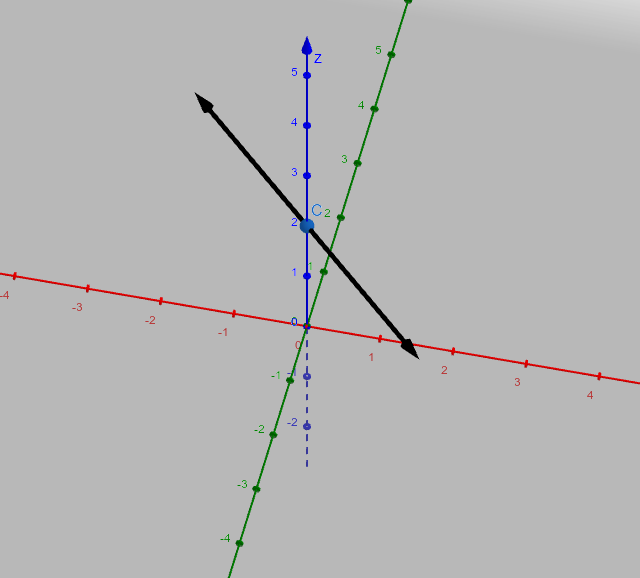
\includegraphics[width=0.3\textwidth]{images/3d-axis-reflection.png}
\end{figure}

\subsubsection{Punkspiegelung}
Für die Punktspiegelung muss für alle Punkte der Gegenvektor zum  Verbindungsvektor von
Spiegelpunkt und zu spiegelndem Punkt gebildet werden. Dieser zeigt dann vom Spiegelpunkt
aus gesehen zur neuen Position des Punktes.
Es verändern sich maximal alle 3 Koordinaten des Punktes.

\subsubsection{Ebenenspiegelung}
Um einen Punkt an einer Ebene zu spiegeln, muss man zuerst den Punkt auf der
Ebene mit dem geringsten Abstand (Lotpunkt) zu diesem bestimmen. Anschließend
spiegelt man den Punkt einfach anhand dieses Punktes. Alternativ kann dies
auch mit einer Geradengleichung (vgl. Lotgerade) realisiert werden.
Es verändert sich maximal 1 Koordinate des Punktes.

\subsubsection{Achsenspiegelung}
Um einen Punkt an einer Achse zu spiegeln, muss man zuerst den Punkt auf der
Achse mit dem geringsten Abstand zu diesem bestimmen (vgl. Punkt-Gerade Abstand).
Anschließend spiegelt man den Punkt einfach anhand dieses Punktes.
Es verändern sich maximal 2 Koordinaten des Punktes.

\subsection{Schnittpunkt von Geraden mit GTR (Matrix, Solve)}

\end{document}
